\documentclass{article}
\usepackage{amsthm,listings,tikz,multicol}
\newtheorem{theorem}{Theorem}
\newenvironment{note}{\begin{quote}\small}{\end{quote}}
\begin{document}
\section{Environments}
\begin{theorem}[Main result]
Every structured unit can be translated independently of its neighbors.
\end{theorem}
\begin{proof}
By construction, each unit carries its own placeholders.
\end{proof}
\begin{center}
Centered prose is part of the section text.
\end{center}
\begin{multicols}{2}
Columns keep their prose in the section.
\end{multicols}
\begin{note}
A custom environment with prose is translated as its own unit.
\begin{itemize}
\item Nested items stay inside the outer environment.
\end{itemize}
\end{note}
\begin{verbatim}
raw   text with 100% literal percent
\end{verbatim}
\begin{lstlisting}[language=Python]
print("50% done")  # not a comment for TeX
\end{lstlisting}
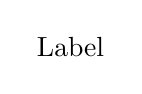
\begin{tikzpicture}
\node {Label};
\end{tikzpicture}
\begin{figure*}
\begin{subfigure}{0.5\linewidth}
\caption{Left panel.}
\end{subfigure}
\end{figure*}
\begin{quote}
Quoted prose with a \verb|%verb%| atom and \url{http://example.com/a_b%20c}.
\end{quote}
\begin{unbalanced}
This environment never ends.
\end{document}
